\chapter{Materials and Methods}

\label{sec:materials}
The materials and methods described in this section present a replication of the study performed
by~\cite{mishra_prediction_2014}. In cases where insufficient details were provided for replication,
these decision points were noted and several sensible options selected and compared. All software 
developed to curate the dataset and perform the experiment, including a Jupyter notebook to reproduce our key results, can be found publicly available on
our GitHub repository: \linkto{https://github.com/big-data-lab-team/reproducibility-bioinfo/}.

\section{Dataset}
\label{sec:dataset}

The SwissProt UniProt database with rich sequence and substrate
annotations~\cite{boeckmann2003swiss} was subsampled to include $900$ membrane transporter proteins and $660$
non-transporter proteins. For the training set, $780$ transport proteins were divided into $7$ substrate-specific 
classes ($70$ amino acid transporters, $60$ anion transporters, $260$ cation transporters, $60$ electron transporters, $60$ 
sugar transporters, $70$ protein/mRNA transporters, and $200$ other transporters). With the addition of 600 non-transporter
proteins, the total dataset contained $1,380$ protein sequences. 

The independent set contains $60$ non-transporter proteins
and the remaining $120$ transporter proteins being divided into the same $7$ substrate-specific classes 
($15$ amino acid transporters, $12$ anion transporters, $36$ cation transporters, $10$ electron transporters, 
$12$ sugar transporters, $15$ protein/mRNA transporters, and $20$ other transporters).

Features were computed for each protein, including: Amino Acid Composition (AAC), Dipeptide Composition (DPC),
Physico-Chemical Composition (PHC), Biochemical Composition (AAindex) and Position-specific scoring matrix (PSSM)
profile. Each feature was computed identically to the methods described by~\cite{mishra_prediction_2014} and are briefly
summarized below:

\begin{itemize}
\item \textbf{Amino Acid Composition (AAC)}: a feature vector of $20$ values ranging from $0$ -- $100$ indicating the
percentage of all standard amino acids present within a protein, as defined by~\cite{gromiha2010protein}. Also known
as Monopeptide Composition (MPC).
\item \textbf{Dipeptide Composition (DPC)}: a feature vector of $400$ values ranging from $0$ -- $100$ indicating the
percentage of all possible ordered amino acid pairs present within a protein, as defined by~\cite{gromiha2010protein}.
\item \textbf{Physico-Chemical Composition (PHC)}: a feature vector of $11$ values corresponding
to percentage composition of physico-chemical residue classes, including: Aliphatic, Neutral, Aromatic, Hydrophobic, Charged, Positively charged,
Negatively charged, Polar, Small, Large, and Tiny. 
\item \textbf{Biochemical Composition (AAindex)}: a feature vector of $49$ physical, chemical, energetic, and
conformational amino acid properties which have been averaged across all amino acids present within the protein.
\item \textbf{Position-specific scoring matrix (PSSM) profile}: a feature vector of $400$ sequence
likelihoods aggregated across min-max scaled probabilities for each ordered amino acid pair within
proteins in the SwissProt database.
\end{itemize}

While the computed AAC, DPC, and PHC features were verified against those previously generated in literature, the 
web reference on the initial study for AAindex and PSSM profiles were not available. So, to validate their similarity 
they were checked with Munira Alballa, a PHD student of Dr. Gregory Butler who was working on related subject \cite{alballa2020trancep}
and was experienced with the matter.


\section{Model Flexibility}
\label{sec:modelflex}
Though the majority of dataset and model specifications were clearly specified by~\cite{mishra_prediction_2014}, there
remains flexibility along various axes in the analysis, namely:

\begin{enumerate}
\item the number of involved classes in the classification task,
\item the sorting and balancing of samples within the dataset,
\item the selected SVM hyperparameters, gamma and cost,
\item the uniformity (or possible lack of) SVM hyperparameters across binary classifiers,
\item the technique applied to aggregation and evaluation of binary classifiers, and
\item the prediction method for the final labels.
\end{enumerate}

Considering the available degrees of freedom and limited computational resources, the AAC feature was used initially
to train and evaluate model parameters. The best performing model using AAC was then re-trained using the full feature
set. In the following section, the experimental design is described in detail with reference to the axes of flexibility,
above. Diagram~\ref{fig:studyProcess} provides a graphic representation of the parameters explored in this
section alongside the process through which the study was conducted.

\section{Experimental Design}
\label{sec:experimentaldesign}
Despite the multi-class nature of this task, the models developed and evaluated below were constructed in a binary
classification scenario. This was accomplished using the ``one versus rest'' strategy which was performed either prior
to training or automatically depending on the classifier. Support Vector Machine (SVM) Classifiers were initially built
using the SVMLight library, originally used by~\cite{mishra_prediction_2014}, which reported a probability of class
membership in each binary setting which were then combined as a multi-class confusion matrix. These models were
replicated using SciKit-learn (SKlearn), a popular library for machine learning in Python, in both an identical setting
to SVMLight (termed: SKlearn Probability) and an approach which automatically performs the class reconstruction and
prediction described above (termed: SKlearn Prediction). 

\subsection{Training}
All models were fit for both $7$ and $8$ class scenarios (Addr: 1) -- excluding and including non-transport proteins,
respectively. The models were fit using $3$ distinct training paradigms: i) balanced, ii) shuffled, and iii)
downsampled (Addr: 2). In the balanced case, training- and testing-sets were created for each model through $5$-fold
cross validation (CV) that were randomly generated and stratified to balance class membership across folds. The
shuffled case was performed similarly to the balanced case without stratification guaranteeing balanced class membership
across folds. The downsampled case was also performed in accordance to the balanced case following a reduction in
samples to $60$ observations per class. This resulted in $6$ distinct training methods.

\subsection{Model Hyperparameters}
For all models, the Radial Basis Function (RBF) kernel was used and the gamma and cost parameters for the model ranged
from $1e^{-5}$ -- $10$ and $1$ -- $4$, respectively, consistent with those presented by~\cite{mishra_prediction_2014}.
Specific values were determined through a grid search (Addr: 3). In the case of SVMLight and SKLearn Probability
scenarios, gamma and cost values were either uniform or varied across classes (Addr: 4), whereas the implementation of
the SKlearn Prediction model permitted only uniform pairs across all classes.

\subsection{Performance Evaluation}
Model performance was evaluated through standard measures of sensitivity, specificity, accuracy, true positives (TP),
false positives (FP), true negatives (TN), false negatives (FN), and Matthew's Correlation Coefficient (MCC) which is a
measure of correlation suitable for imbalanced classification problems~\cite{mcc2017optimal}. As micro- and
macro-averaging approaches -- evaluating binary classifiers before or after aggregation into a multi-class model,
respectively -- lead to different results in an imbalanced classification setting, both approaches were used for
scoring here (Addr: 5).

In the case of both the SVMLight and SKlearn Probability models, the resulting classification and performance for each
model was determined by the aggregation of independent binary classifiers according to three distinct methods: maximum
probability, unweighted average, and balanced average (Addr: 6). The maximum probability method assigns each sample a
label corresponding to the binary classifier with the highest certainty, resulting in a non-overlapping classification
result which was evaluated. In the case of both averaging methods, each probability is converted into a binary
classification through thresholding and is scored independently prior to aggregating the performance of all classifiers.
The unweighted average thresholds probabilities at the median value, whereas the balanced case uses a threshold
proportional to the true number of members belonging to a given class. As the SKlearn Prediction model returned
pre-determined group confusion matrix and class memberships, performance metrics were computed upon these directly.

\section{Model Comparison}
Models were compared to the reported reference classifier through the Euclidean distance between a 4-dimensional
feature vector containing Sensitivity, Specificity, Accuracy, and MCC. The closest models were chosen as those which
minimized this distance. Model settings, such as those defined to address points 1 -- 6 above, were compared
quantitatively through the pairwise application of two-sided Mann–Whitney U Tests on the distribution of distance
values for all unique settings within a given category (i.e. the distribution of distances for all models using
micro-averaging was compared to the equivalent distribution for all models using macro-averaging). To avoid
overfitting, the closest 10\% of models to the reference were selected as the models used for further investigation.

\begin{figure}[ht]
    \centering
    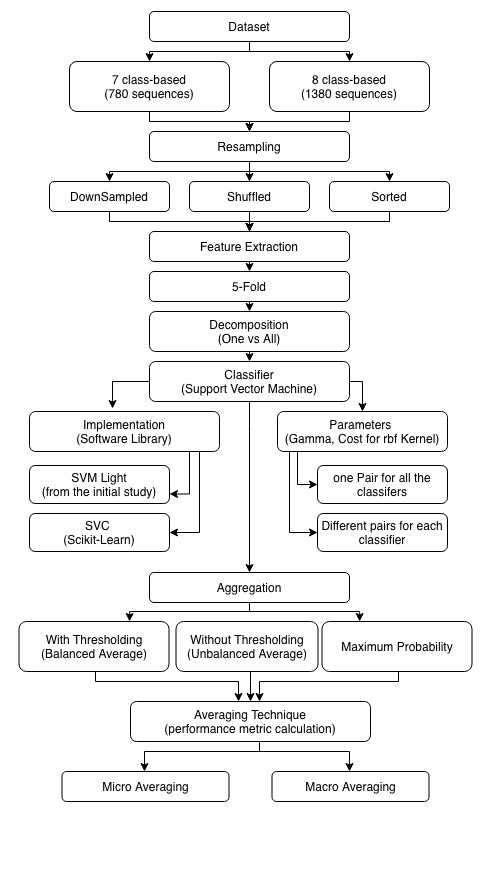
\includegraphics[width=0.80\textwidth]{figures/13studyProcess.jpg}
    \caption{The study process}
    \label{fig:studyProcess}
\end{figure}